\documentclass[3pt,twocolumn]{elsarticle}
\usepackage[spanish]{babel}
\usepackage[utf8]{inputenc}
\usepackage[hidelinks]{hyperref}
\usepackage{graphics}
\usepackage{graphicx}
\usepackage{epsfig}
\usepackage{amssymb}
\usepackage{amsmath}
\usepackage{amsthm}
\usepackage{lineno}
\usepackage{tikz}
\usepackage{float}
\usepackage{subcaption}
\usepackage{amssymb, amsmath}
\usetikzlibrary{shapes,arrows}
\usepackage{pstricks,pst-node,pst-tree}
\bibliographystyle{elsarticle-num}

\makeatletter
\renewenvironment{abstract}{\global\setbox\absbox=\vbox\bgroup
\hsize=\textwidth\def\baselinestretch{1}%
\noindent\unskip\textbf{Resumen} % <--- Edit as necessary
\par\medskip\noindent\unskip\ignorespaces}
{\egroup}

\def\keyword{%
\def\sep{\unskip, }%
\def\MSC{\@ifnextchar[{\@MSC}{\@MSC[2000]}}
\def\@MSC[##1]{\par\leavevmode\hbox {\it ##1~MSC:\space}}%
\def\PACS{\par\leavevmode\hbox {\it PACS:\space}}%
\def\JEL{\par\leavevmode\hbox {\it JEL:\space}}%
\global\setbox\keybox=\vbox\bgroup\hsize=\textwidth
\normalsize\normalfont\def\baselinestretch{1}
\parskip\z@
\noindent\textit{Palabras clave: } % <--- Edit as necessary
\raggedright % Keywords are not justified.
\ignorespaces}

\biboptions{longnamesfirst,comma}


\makeatother
\begin{document}

\twocolumn[
\begin{@twocolumnfalse}

\begin{frontmatter}
\title{Dinamica Molecular 3D de un líquido por el metodo de Verlet con el potencial de Lenard-Jones}
\author{Llano, G. A}
\address{Facultad de Ingeniería Mecánica y Eléctrica, Universidad Autónoma de Nuevo León}

\begin{abstract}

El uso de la simulación por dinámica molecular es un tipo de simulación donde es posible el estudio de las interacciones moleculares de algún material ya sea en estado líquido, solido o gaseosos, que permite el análisis de diferentes parámetros para el estudio de alguna propiedad específica, esto se integra por medio del algoritmo de Verlet resolviendo las ecuaciones de movimiento de newton donde es posible aplicar un potencial conocido como Lennard-Jones que se aplica en conjunto con lo anterior para el estudio de diferentes propiedades fisicoquímicas de los materiales.

\end{abstract}
\begin{keyword}
Dinámica Molecular \sep Lennard-Jones \sep Verlet \sep Nanotecnología
\end{keyword}

\end{frontmatter}
\end{@twocolumnfalse}
]

\section{Introducción}\label{intr}
La interacción entre partículas es un tema de estudio capas de aplicarse para diferentes situaciones en el desarrollo de nuevos materiales, aplicado para conocer ciertas características fisicoquímicas de alguna molécula en específico, en donde se toman en cuenta las fuerzas tanto de atracción como repulsión así como la interacción entre estas, una manera sencilla de visualizarlas es mediante una simulación computacional por dinámica molecular \cite{LDIM} en la que se toman en cuenta diversos parámetros para poder llevar con éxito dicha simulación, que va desde parámetros físicos como la descripción de la molécula, en número de partículas o el número de iteraciones en el sistema, hasta lo más complejo que es la aplicación de modelos y potenciales de tal manera que sea más realista la simulación dejando de lado el simple potencial gravitacional, añadiendo diversas subrutinas donde se aplique un potencial diferente así como un modelo tal como el de Verlet, para poder integrar la resolución de ecuaciones del movimiento donde nos brindan diferentes parámetros, como las diferentes energías, o temperaturas de un sistema en cuestión así como diversas características fisicoquímicas, en el presente trabajo se busca realizar una simulación por dinámica molecular de un líquido en el cual se utilice el potencial de Lennard-Jones así como la integración del modelo de Verlet, de tal manera de obtener un modelo en 3D . Los principales objetivos se describen a continuación:

\begin{itemize}
\item Definir parámetros para simular la molécula del agua.
\item Las moléculas se encuentren en un espacio delimitado así mismo no salgan de este
\item Que estas interactúen aplicando el potencial de Lennard-Jones
\item Crear una rutina de tal manera que al momento que estas interactúen no choquen que exista un potencial, y así mismo si estas se llegasen a juntar las moléculas no se sobrepongan.
\item Aplicar el modelo de Verlet de tal manera que sea posible el cálculo de aceleraciones y velocidades en trabajos futuros
\item Poder obtener una visualización en 3D
\end{itemize}

Primeramente, se describirá algunos conceptos básicos para tener en claro cómo es que se lleva a cabo este tipo de simulación así mismo se define la metodología utilizada, herramientas, así como los resultados y conclusiones del presente trabajo.


\section{Antecedentes}\label{antesc}

Actualmente existen diferentes técnicas de simulación computacional donde es posible crear alguna simulación de diversos fenómenos de interés, que van desde lo más simple hasta lo más complejo, en cuanto a la nanotecnología se aprovechan diversas herramientas de simulación computacional para observar dichos fenómenos, se sabe que la nanotecnología se define \cite{nano} como el estudio y manipulación de la materia a escala nanométrica es decir de 1 a 100 nm particularmente hablando de átomos y moléculas, donde fenómenos como la interacción entre partículas y/o moléculas generan un gran interés para el estudio y el desarrollo de nuevos materiales.

Generalmente este tipo de interacciones a escala molecular en donde es posible analizar el movimiento de las partículas observadas por medio de técnicas de simulación son conocidas como dinámica molecular o simulación por dinámica molecular \cite{Dm, DMA}. Este tipo de simulación se emplea aprovechando las leyes de newton del movimiento para el análisis del comportamiento del sistema en cuestión a través del tiempo donde es posible calcular las fuerzas entre los átomos que conforman dicho sistema, al aplicarse las leyes del movimiento de newton se pueden generar trayectorias en un sistema compuesto por $N$ partículas mediante integración numérica directa a dichas ecuaciones, específicamente tratándose de la segunda ley de newton la cual es la encargada de cuantificar lo que conocemos como fuerza, donde la aceleración que adquiere un cuerpo es directamente proporcional a la fuerza neta aplicada sobre el mismo \cite{new, Dm}.

\subsection{Dinámica molecular}

El uso de la simulación por dinámica molecular permite obtener diferentes propiedades fisicoquímicas de un sistema de energía libre como son la entropía, viscosidad, temperatura de cambio de fase, presión, energía cinética, energía potencial etc., así mismo es posible su aplicación en fenómenos de carácter biológico, permitiendo medir las fuerzas de interacción entre algún fármaco y sus receptores o células blanco \cite{revist}. Hablando en términos de la dinámica molecular su mayor aplicación radica en la descripción de la solución de las ecuaciones clásicas del movimiento anterior mente mencionadas, las leyes de newton aplicadas en un conjunto de átomos o moléculas analizando sistemas que se encuentren en equilibrio o bien fuera de equilibrio. 

La simulación por dinámica molecular \cite{DMA} tuvo sus inicios en 1956 cuando Alder y Wainwright estudiaron la dinámica de un conjunto de esferas duras, posteriormente en 1959 se realizó el primer análisis por medio de dinámica molecular para un material real, el cual fue publicado hasta 1960 en el cual se estudió el daño por radiación en cobre cristalino, posteriormente se aplicó la dinámica molecular para el estudio de un material liquido en 1964 años más tarde se comenzaron a aplicar métodos para el estudio de sistemas que se encontraban fuera de equilibrio con el fin de poder medir coeficientes de transporte, como son conductividad térmica o bien coeficiente de difusión entre otros. 

\subsection{Metodología de la simulación por DM}
Generalmente la simulación por medio de dinámica molecular se realiza en cuatro etapas \cite{revist,Dm}, las cuales son:

\begin{itemize}
\item Preparación del sistema.
\item Equilibramiento.
\item simulación por DM.
\item Resultados.
\end{itemize}


En donde primeramente se describe el sistema con el cual se va a trabajar, se definen los parámetros iniciales número de partículas o moléculas y características específicas como el modelo de las interacciones del ambiente-sistema, así como el desarrollo de ecuaciones de movimiento.

En la etapa de equilibramiento se realiza utilizando esquemas o ensambles de simulación como, ensamble canónico. Supercanonico, micro canónico, isobárico, o isotérmico etc., se equilibra el sistema de tal manera que la energía permanece casi constante esto dependiendo del esquema o ensamble con el que se trabaja, en esta etapa también se definen condiciones constantes en cuanto a presión, temperatura, y energía. 

En la etapa de simulación se define el tiempo de ejecución (pasos o iteraciones), se resuelven las ecuaciones de movimiento corriendo la dinámica molecular, aquí se realiza el cálculo de fuerzas del sistema por el cual se obtienen las propiedades fisicoquímicas de interés. Y finalmente en resultados se analizan los datos de interés obtenidos, así mismo se puede realizar algún otro calculo por medio del ensamble que se utiliza, o para una mejor visualización se analiza el comportamiento del sistema con el apoyo de imágenes, o alguna animación.


\subsection{Interacciones moleculares}
El cálculo en las interacciones moleculares es utilizado para representar tanto las fuerzas de atracción como las fuerzas de repulsión. Este tipo de interacción moleculares son capaces de representarse a través de la energía potencial \cite{revist,docM},una manera de aproximación aplicada es descomponiendo tal energía de manera que se involucran las interacciones de pares o tripletes de átomos, en este caso se aplican potenciales tales como Lennard-Jones el cual fue desarrollado con la finalidad de obtener un análisis en cuanto al comportamiento atómico en gases y actualmente aplicado también en líquidos.


\subsection{Lennard-jones}
El potencial de Lennard-Jones \cite{LJN} fue propuesto en 1924, en esta gobierna la fuerza de interacción y la repulsión de un par de átomos $i$ y $j$ ubicados en las posiciones $ri$ y $rj$. Bajo el cual se calculan las aceleraciones y fuerzas en función de la distancia de separación $r$.

\begin{equation}
u(rij)=4 \epsilon[ (\frac{\sigma}{rij} )^{12} - (\frac{\sigma}{rij} )^6]
\end{equation}

Este modelo es conformado por las fuerzas repulsivas $(\frac{\sigma}{rij} )^{12}$ como atractivas $(\frac{\sigma}{rij} )^6$ 
El parámetro $r$ es la distancia entre los dos átomos, $\sigma$ es una escala de la longitud que representa la distancia a la que el potencial intermolecular entre los átomos es igual a $0$ así $\epsilon$ este dado por la fuerza de interacción en unidades de $eV$, como tal es una medida de fuerza bajo la cual dos átomos son atraídos entre sí. Al aplicarse este potencial a una simulación por dinámica molecular, se hace la integración de las ecuaciones del movimiento mediante diferentes tipos de algoritmos más común usado el algoritmo de Verlet el cual su principio parte de la resolución a las ecuaciones de movimiento aplicadas para cada una de las partículas que interactúan mediante fuerzas intermoleculares en donde la suma de todas las interacciones de las partículas dará como resultado la fuerza neta del sistema \cite{docM,LJN}.


\section{Trabajos relacionados}\label{intr}

Schaeffer \cite{elisa} propuso un modelo de interacción entre partículas visualizado en $2D$ en donde es aplicado un potencial gravitacional, bajo el cual es posible visualizar la interacción entre las partículas, así como ver la predominancia de las fuerzas que interactúan entre sí, a partir de este modelo es posible una simulación tanto $2D$ como $3D$ donde en lugar de aplicar un potencial gravitacional se aplique el potencial de Lennard-Jones, simulando algún compuesto en específico.
Así mismo Morales \cite{docM} aplica el algoritmo de Verlet en conjunto con el potencial de Lennard-Jones para el cálculo y simulación de sus diferentes aplicaciones como son el tiro parabólico, la simulación de una partícula libre, el cálculo de las fuerzas de fricción y la simulación de un gas ideal tanto en $2D$ como en $3D$.

\section{Experimentación }\label{intr}

La simulación se realizó en una laptop Lenovo modelo ideapad 330-14IGM con un procesador Intel(R) Celeron(R) n4000 CPU 1.10GHz, haciendo uso del software Python \cite{python} versión 3.7. Partiendo como base del código propuesto por Schaeffer \cite{elisa} sobre la interacción de partículas, modificando el potencial gravitacional por el de Lennard-Jones así mismo aplicando el modelo de Verlet, para realizar la interacción de un líquido en este caso el agua, con un modelo 3D buscando que tal simulación cumpla con distintos parámetros.
\begin{itemize}
\item Definir parámetros para simular la molécula del agua.
\item Las moléculas se encuentren en un espacio delimitado así mismo no salgan de este
\item Que estas interactúen aplicando el potencial de Lennard-Jones
\item Crear una rutina de tal manera que al momento que estas interactúen no choquen que exista un potencial, y así mismo si estas se llegasen a juntar las moléculas no se sobrepongan.
\item Aplicar el modelo de verlet de tal manera que sea posible el cálculo de aceleraciones y velocidades en trabajos futuros
\item Poder obtener una visualización en 3D
\end{itemize}


\section{Resultados y discusiones}\label{intr}

Buscando cumplir los puntos anteriormente mencionados se incorporaron diversas rutinas para poder cumplir cada uno de estos, se definieron los parámetros físicos como es el número de partículas que en este caso fueron $64$, así como el número de iteraciones que fueron $100000$, se dio la masa de la partícula del agua, así como la densidad y el radio de esta, se utilizó la librería Vpython para poder obtener la visualización en $3D$.
Entre los puntos mencionados se buscaba que las partículas no chocaran entre sí, no se sobrepongan, así como se encuentren en un espacio delimitado, y que se ejerza el potencial de Lennard-jones.


En la figura \ref{f1} se observa que las $64$ partículas efectivamente se encontraban en el espacio delimitado así mismo demostrando la simulación en 3D esto se logró con la rutina “def anint” \cite{ana} logrando que las partículas no se salieran de la caja.


\begin{figure}[h!]
\centering
\begin{subfigure}[b]{0.65\linewidth}
\includegraphics[width=\linewidth]{Sim1 (17).png}
\caption{Vista aerea.}
\label{f1.1}
\end{subfigure}
\begin{subfigure}[b]{0.65\linewidth}
\includegraphics[width=\linewidth]{Sim1 (14).png}
\caption{Vista frontal}
\label{f1.2}
\end{subfigure}
\caption{Simulación en 3D, con área delimitada.}
\label{f1}
\end{figure}


En la figura \ref{f2} se observa que estas no se sobreponían entre sí que era uno de los objetivos buscados, esto se logró con la incorporación de la rutina “def choques” \cite{ana}.

\begin{figure}[h!]
\centering
\begin{subfigure}[b]{0.65\linewidth}
\includegraphics[width=\linewidth]{Sim1 (33).png}
\caption{interacción de partículas.}
\label{f2.1}
\end{subfigure}
\begin{subfigure}[b]{0.65\linewidth}
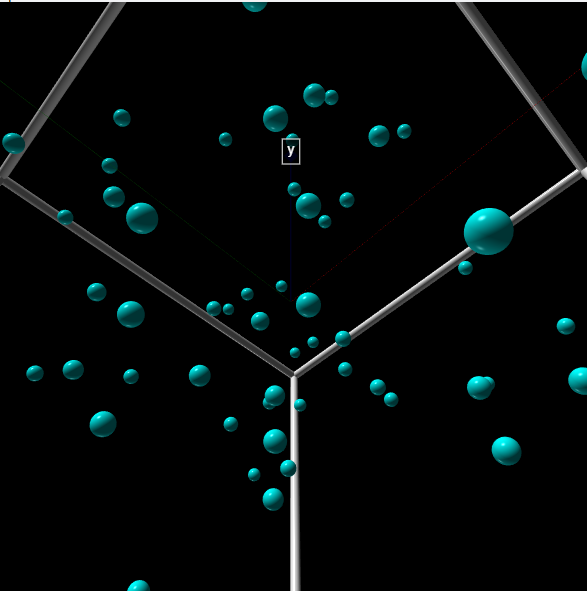
\includegraphics[width=\linewidth]{Sim1 (34).png}
\caption{Acercamiento de la interacción.}
\label{f2.2}
\end{subfigure}
\caption{interacción de las partículas vista de diferentes ángulos}
\label{f2}
\end{figure}


Así mismo uno de los puntos más importantes fue que la interacción entre partículas se diera por medio del potencial de Lennard-Jones, tal potencial se observa de manera gráfica en la figura \ref{f3}.

\begin{figure}[h!]
\centering
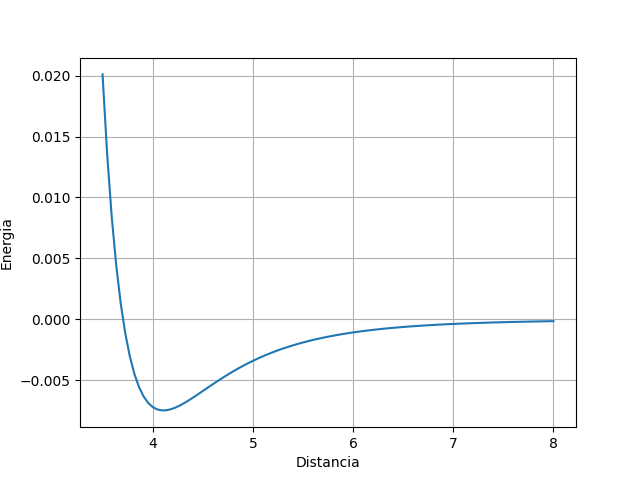
\includegraphics[width=\linewidth]{Lennard-Jones.png}
\caption{Potencial de Lennard-Jones.}
\label{f3}
\end{figure}

\begin{figure}[h!]
\centering
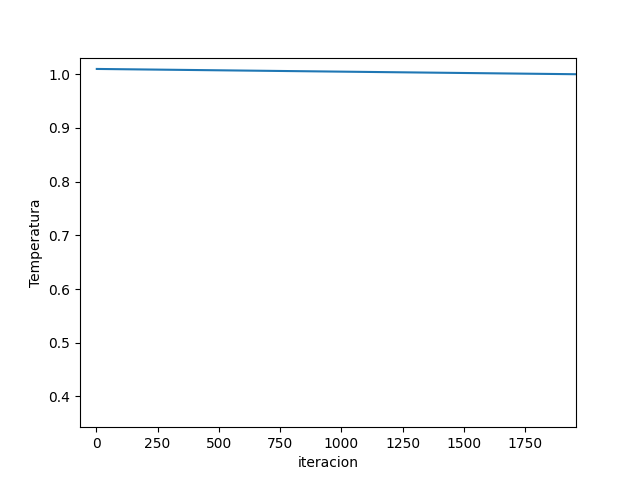
\includegraphics[width=\linewidth]{canonico itervs temp.png}
\caption{Demostración de ensamble tipo canonico.}
\label{f4}
\end{figure}

Se utilizo otra subrutina “def termalización” \cite{ana} en donde aplicando las leyes de newton su función seria calcular la temperatura del sistema donde la energía presente se transforma en temperatura en la figura \ref{f4} se puede observar las temperaturas en donde se observa que la simulación en cuestión es de tipo ensamble canónico en donde la energía así como la temperatura permanece casi constante durante todas las iteraciones así mismo se utiliza el algoritmo de Verlet, que es parte principal de la simulación donde se calculan las velocidades y aceleraciones actualizando las posiciones en cada iteración. Misma se observa en la figura \ref{f5} el tiempo de cálculo de la computadora por cada iteración, en esta se puede observar que cuando va aproximadamente en la mitad de las iteraciones al equipo utilizado le toma un poco más de trabajo el poder realizar los cálculos.

\begin{figure}[h!]
\centering
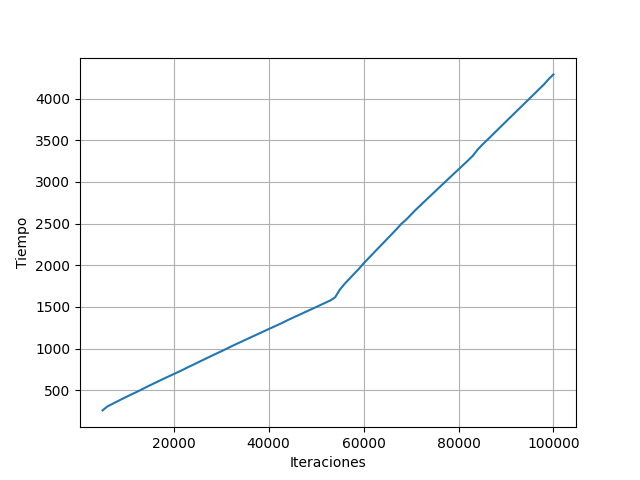
\includegraphics[width=\linewidth]{tiempocalculo.png}
\caption{Tiempo de cálculo del sistema por iteración.}
\label{f5}
\end{figure}

\section{Conclusiones}\label{intr}
Se realizo una simulación por dinámica molecular con tipo de ensamble canónico, aplicado el potencial de Lennard-Jones donde la parte principal fue la incorporación del algoritmo de Verlet, para el cálculo de las posiciones, se observó que es posible realizar una simulación en $3D$ de alguna molécula en específico en este caso la del agua, mediante el uso de este tipo de simulación es posible la obtención de más datos como son las energías cinéticas, potencial, temperaturas del sistema entre otras, que pueden ser muy bien aprovechadas cuando se estudia algún material en específico, ya que el conocer la interacción entre moléculas o partículas se puede aprovechar para conocer diferentes parámetros entre estos el comportamiento que puede llegar a tener algún material en un medio especifico.
Así mismo en la figura \ref{f6} se observa dicha simulación vista por diferentes ángulos.


\begin{figure}[h!]
\centering
\begin{subfigure}[b]{0.45\linewidth}
\includegraphics[width=\linewidth]{Sim1 (32).png}
\caption{a}
\label{f6.1}
\end{subfigure}
\begin{subfigure}[b]{0.45\linewidth}
\includegraphics[width=\linewidth]{Sim1 (8).png}
\caption{b}
\label{f6.2}
\end{subfigure}
\begin{subfigure}[b]{0.45\linewidth}
\includegraphics[width=\linewidth]{Sim1 (28).png}
\caption{c}
\label{f6.3}
\end{subfigure}
\begin{subfigure}[b]{0.45\linewidth}
\includegraphics[width=\linewidth]{Sim1 (19).png}
\caption{d}
\label{f6.4}
\end{subfigure}
\caption{Simulacion en 3D, vista de diferentes angulos.}
\label{f6}
\end{figure}


\subsection{Trabajos futuros}
Se pueden describir un sinfín de trabajos futuros debido a la variedad de aplicaciones que este tipo de simulación proporcionan, algunos de estos serían los siguientes.
Debido a las características del equipo no se pudo realizar una versión paralelizada de tal manera que se pudiera optimizar dicha simulación, se obtuvieron los tiempos de cálculo, pero un trabajo a futuro sería el realizar su versión paralelizada en algún equipo de mejores características que el utilizado y de tal manera poder comparar con los tiempos de cálculo del equipo para la optimización de este.
Otro trabajo a futuro seria modificar el tipo de ensamble utilizado, en este caso fue uno canónico, y sería el utilizar un ensamble tipo gran canónico de tal manera que se utilice la energía potencial del sistema para poder realizar más cálculos, así mismo la modificación de los parámetros físicos de tal manera de no simular agua sino más bien algún otro material de interés.


\bibliography{Pfinal}

\end{document}
